\documentclass{beamer}

\usetheme{Madrid}
\setbeamertemplate{navigation symbols}{}
\setbeamertemplate{footline}[frame number]
\usepackage{graphicx}
\graphicspath{{figures/}}

\title{Hedging Against Turkish Inflation}
\author{Selin Acar, Necati Furkan Çolak, Denis Lasser}
\date{December 2024}

% Bibliography setup
\usepackage[round]{natbib}
\bibliographystyle{plainnat}
\setbeamertemplate{bibliography item}[text]

\begin{document}

% Title Page
\frame{\titlepage}

% Table of Contents
\begin{frame}{Outline}
\tableofcontents
\end{frame}

% Introduction I
\section{Introduction}
\begin{frame}{Introduction I}
\begin{itemize}
\item Ongoing economic crisis in Türkiye has been characterized by
\textbf{high inflation}, the \textbf{depreciation of the Turkish Lira}
(TRY), \textbf{rising borrowing costs}, and \textbf{increasing loan
defaults}.
\item The underlying causes of the crisis can be attributed to
\textbf{political instability}, \textbf{global economic pressures},
and the implementation of \textbf{unconventional economic policies}.
\item Since 2018, inflation has been a persistent issue, partly due to
fluctuations in global oil prices and exchange rates, with
\textbf{Turkey's inflation rate ranking among the highest in emerging
markets} \citep{yilmazkuday_2022}.
\end{itemize}
\end{frame}

% Introduction II
\begin{frame}{Introduction II}
\begin{itemize}
\item The Turkish government's policy of maintaining low interest rates to
stimulate growth, despite the conventional theory that raising
interest rates should reduce inflation, has contributed significantly
to the current economic challenges \citep{kantur_ozcan_2021}.
\item Interest rates have been raised significantly. The most recent rate
hike was in March 2024, when the central bank increased the
\textbf{interest rate} by 5 percentage points to \textbf{50\%} as the
year-on-year inflation reached 75\% \citep{bloomberg_2024}.
\item Since then, the rate has remained unchanged as the central bank has
been committed to fighting high inflation and stabilising the Turkish
lira. As of October 2024, \textbf{year-on-year inflation stands at
48\%} \citep{bloomberg_2024}.
\end{itemize}
\end{frame}

% Methodology I
\section{Methodology}
\subsection{Analyze Asset Performance}
\begin{frame}{Methodology I: Analyze Asset Performance}
\begin{itemize}
\item Analyze asset performance using monthly data (Jan 2018--Sep 2024).
\item Two steps:
\begin{enumerate}
\item Evaluate individual asset hedging effectiveness.
\item Construct an optimal hedging portfolio using Markowitz optimization.
\end{enumerate}
\end{itemize}
\end{frame}

% Methodology II
\subsection{Data Sources}
\begin{frame}{Methodology II: Data Sources}
\begin{itemize}
\item From Bloomberg:
\begin{itemize}
\item \textbf{TUCXEFYY Index}: Turkish core CPI (excluding food, energy,
alcohol, tobacco).
\item \textbf{XU100 Index}: Turkish stock index (BIST 100).
\item \textbf{GTTRY10YR}: 10-Year Turkish Government Bond.
\item \textbf{XAU}: Global prices in USD. 
\item \textbf{XBT BGN}: Bitcoin prices in USD.
\end{itemize}
\item From Turkish Central Bank:
\begin{itemize}
\item \textbf{TP KFE TR-1}: Turkish house price index.
\end{itemize}
\end{itemize}
\end{frame}

% Methodology III
\subsection{Excess Return}
\begin{frame}{Methodology III: Excess Return}

\begin{itemize}
\item The first step is to calculate the real return for each asset relative to the Turkish inflation rate. 
\item Ensures a consistent measure of an asset's effectiveness in preserving purchasing power in Türkiye's inflationary environment.
\end{itemize}

\[
\text{Real Return} = \frac{1 + \text{Nominal Return}}{1 + \text{Inflation Rate}} - 1
\]
\end{frame}

% Methodology IV
\subsection{Markowitz Optimization}
\begin{frame}{Methodology IV: Markowitz Optimization}
\begin{itemize}
\item Building on the individual asset analysis: Markowitz portfolio optimization to construct an optimal portfolio that maximizes the hedging effectiveness against Turkish inflation.
\item Portfolio return: \[
R_p = \sum_{i=1}^{n} w_i R_i
\]
\item Portfolio variance: \[
\sigma_p^2 = \sum_{i=1}^{n} \sum_{j=1}^{n} w_i w_j \sigma_{ij}
\]
\item Minimize portfolio risk: \[
\min_{w} \, \sigma_p^2 \quad \text{subject to:} \quad \sum_{i=1}^{n} w_i R_i = R_{\text{target}}, \quad \sum_{i=1}^{n} w_i = 1, \quad w_i \geq 0
\]
\end{itemize}
\end{frame}

% Results: Individual Assets
\section{Results}
\begin{frame}{Results: Turkish Stocks}
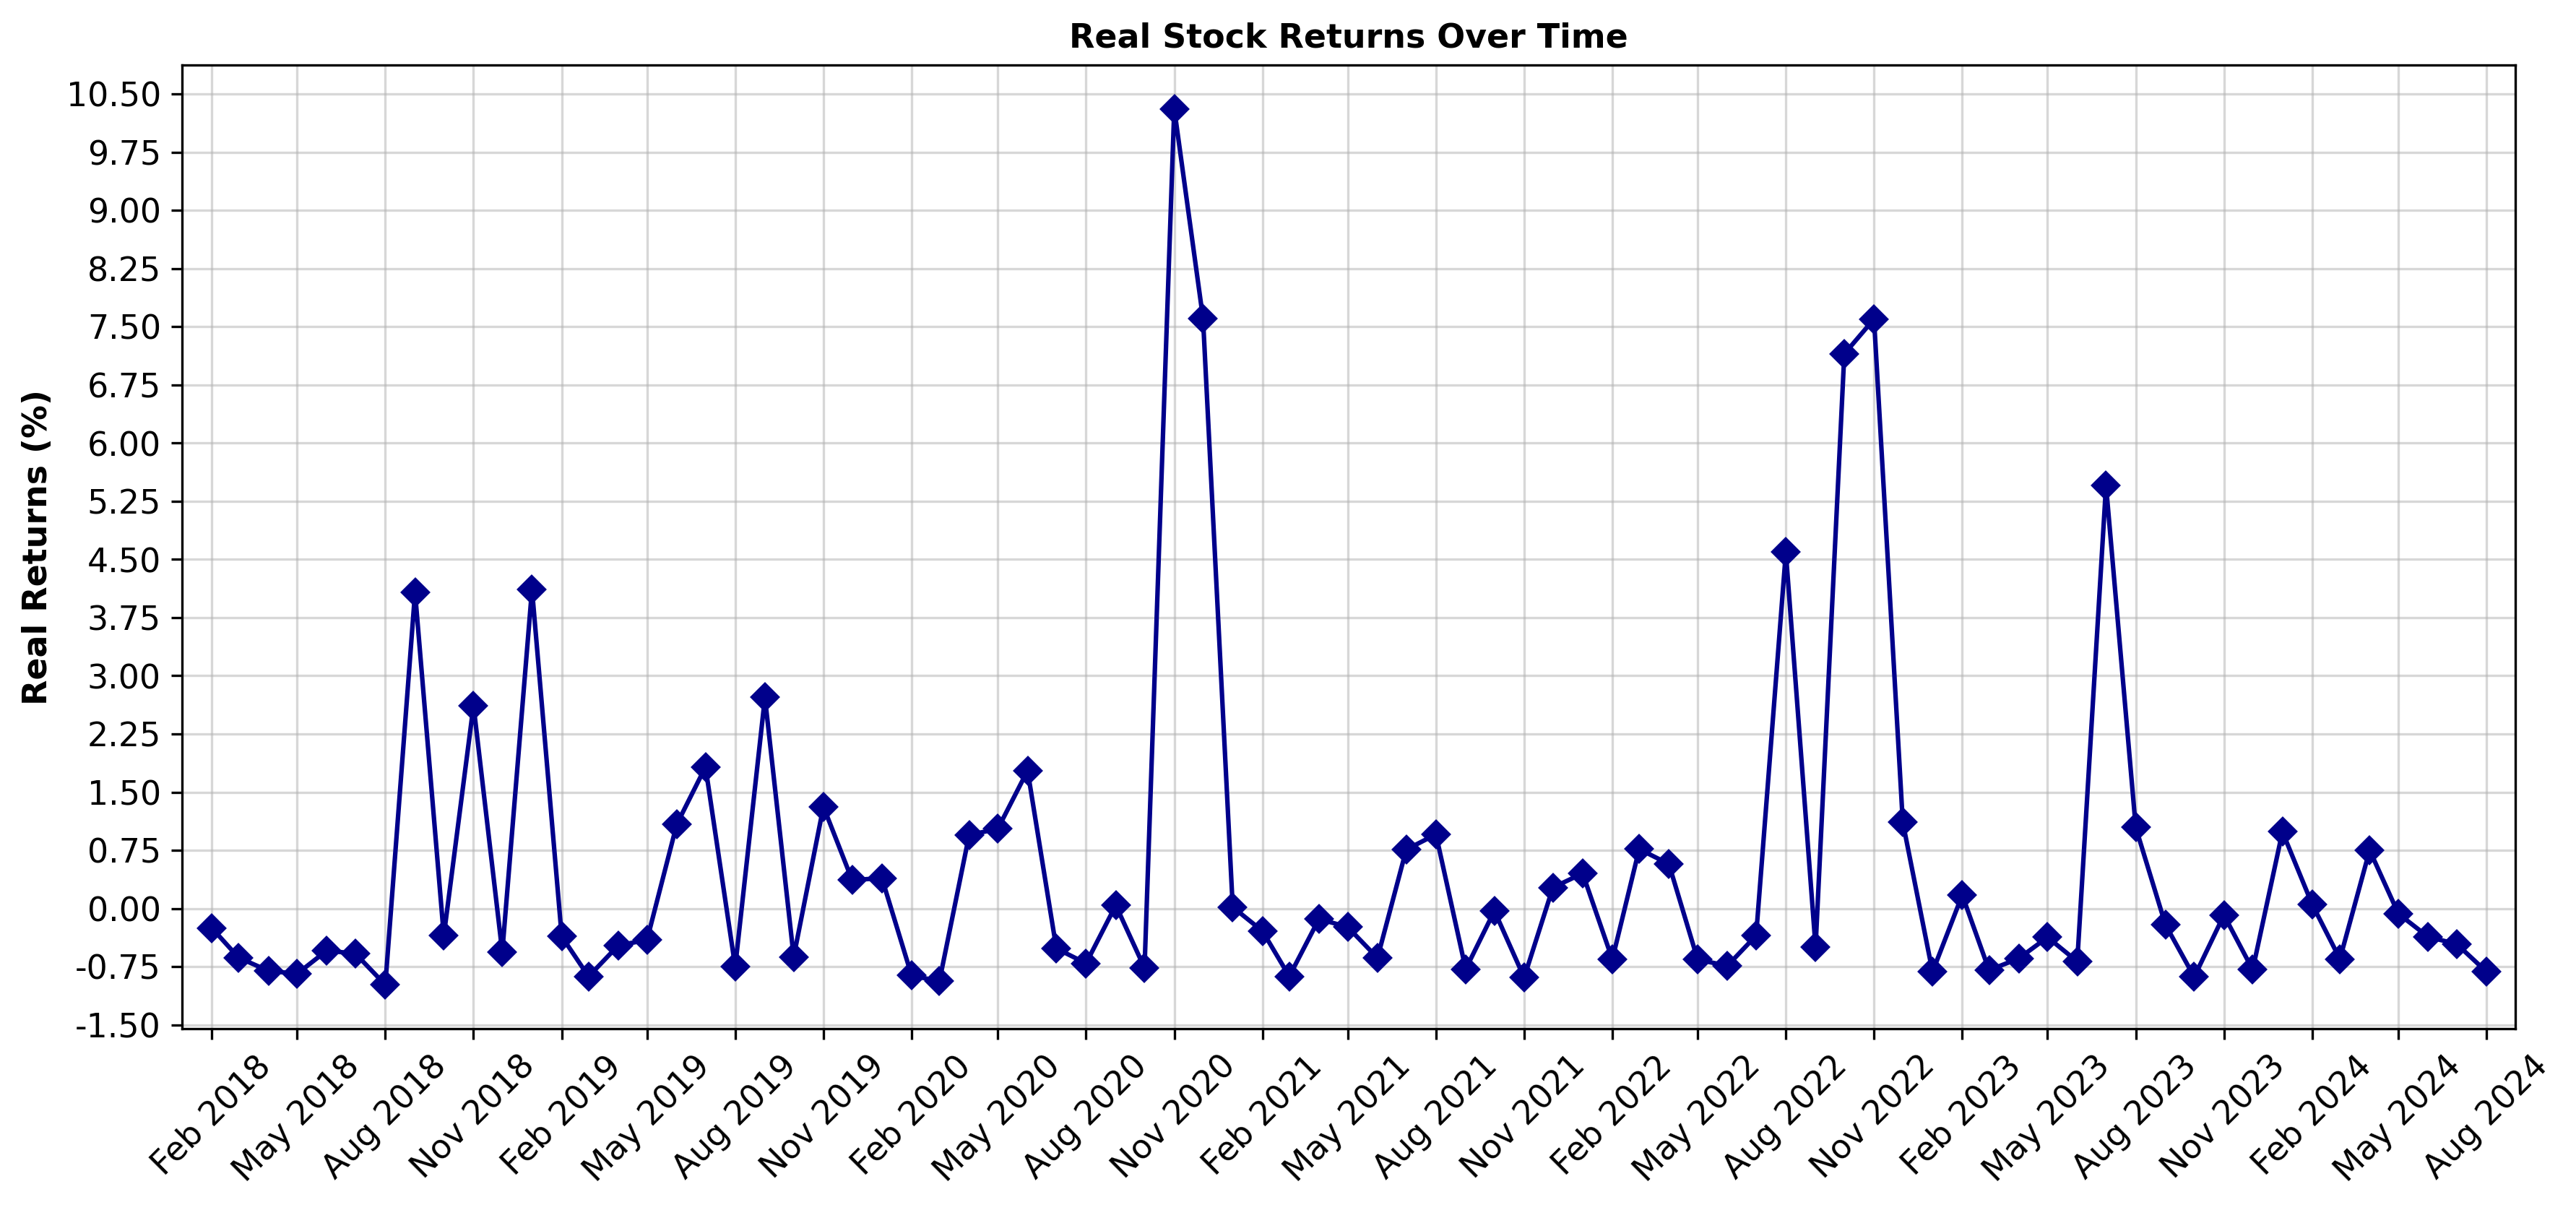
\includegraphics[width=0.7\textwidth]{real_stock_returns.png}
\begin{itemize}
\item Turkish stocks are highly volatile with several sharp peaks and periods of low or negative returns.
\item Turkish equities appear to offer opportunities for inflation hedging during certain periods, but are inconsistent as a hedge.
\item Stocks may reflect market optimism during inflationary periods, they still carry significant risks.
\end{itemize}
\end{frame}

\begin{frame}{Results: Turkish Government Bond}
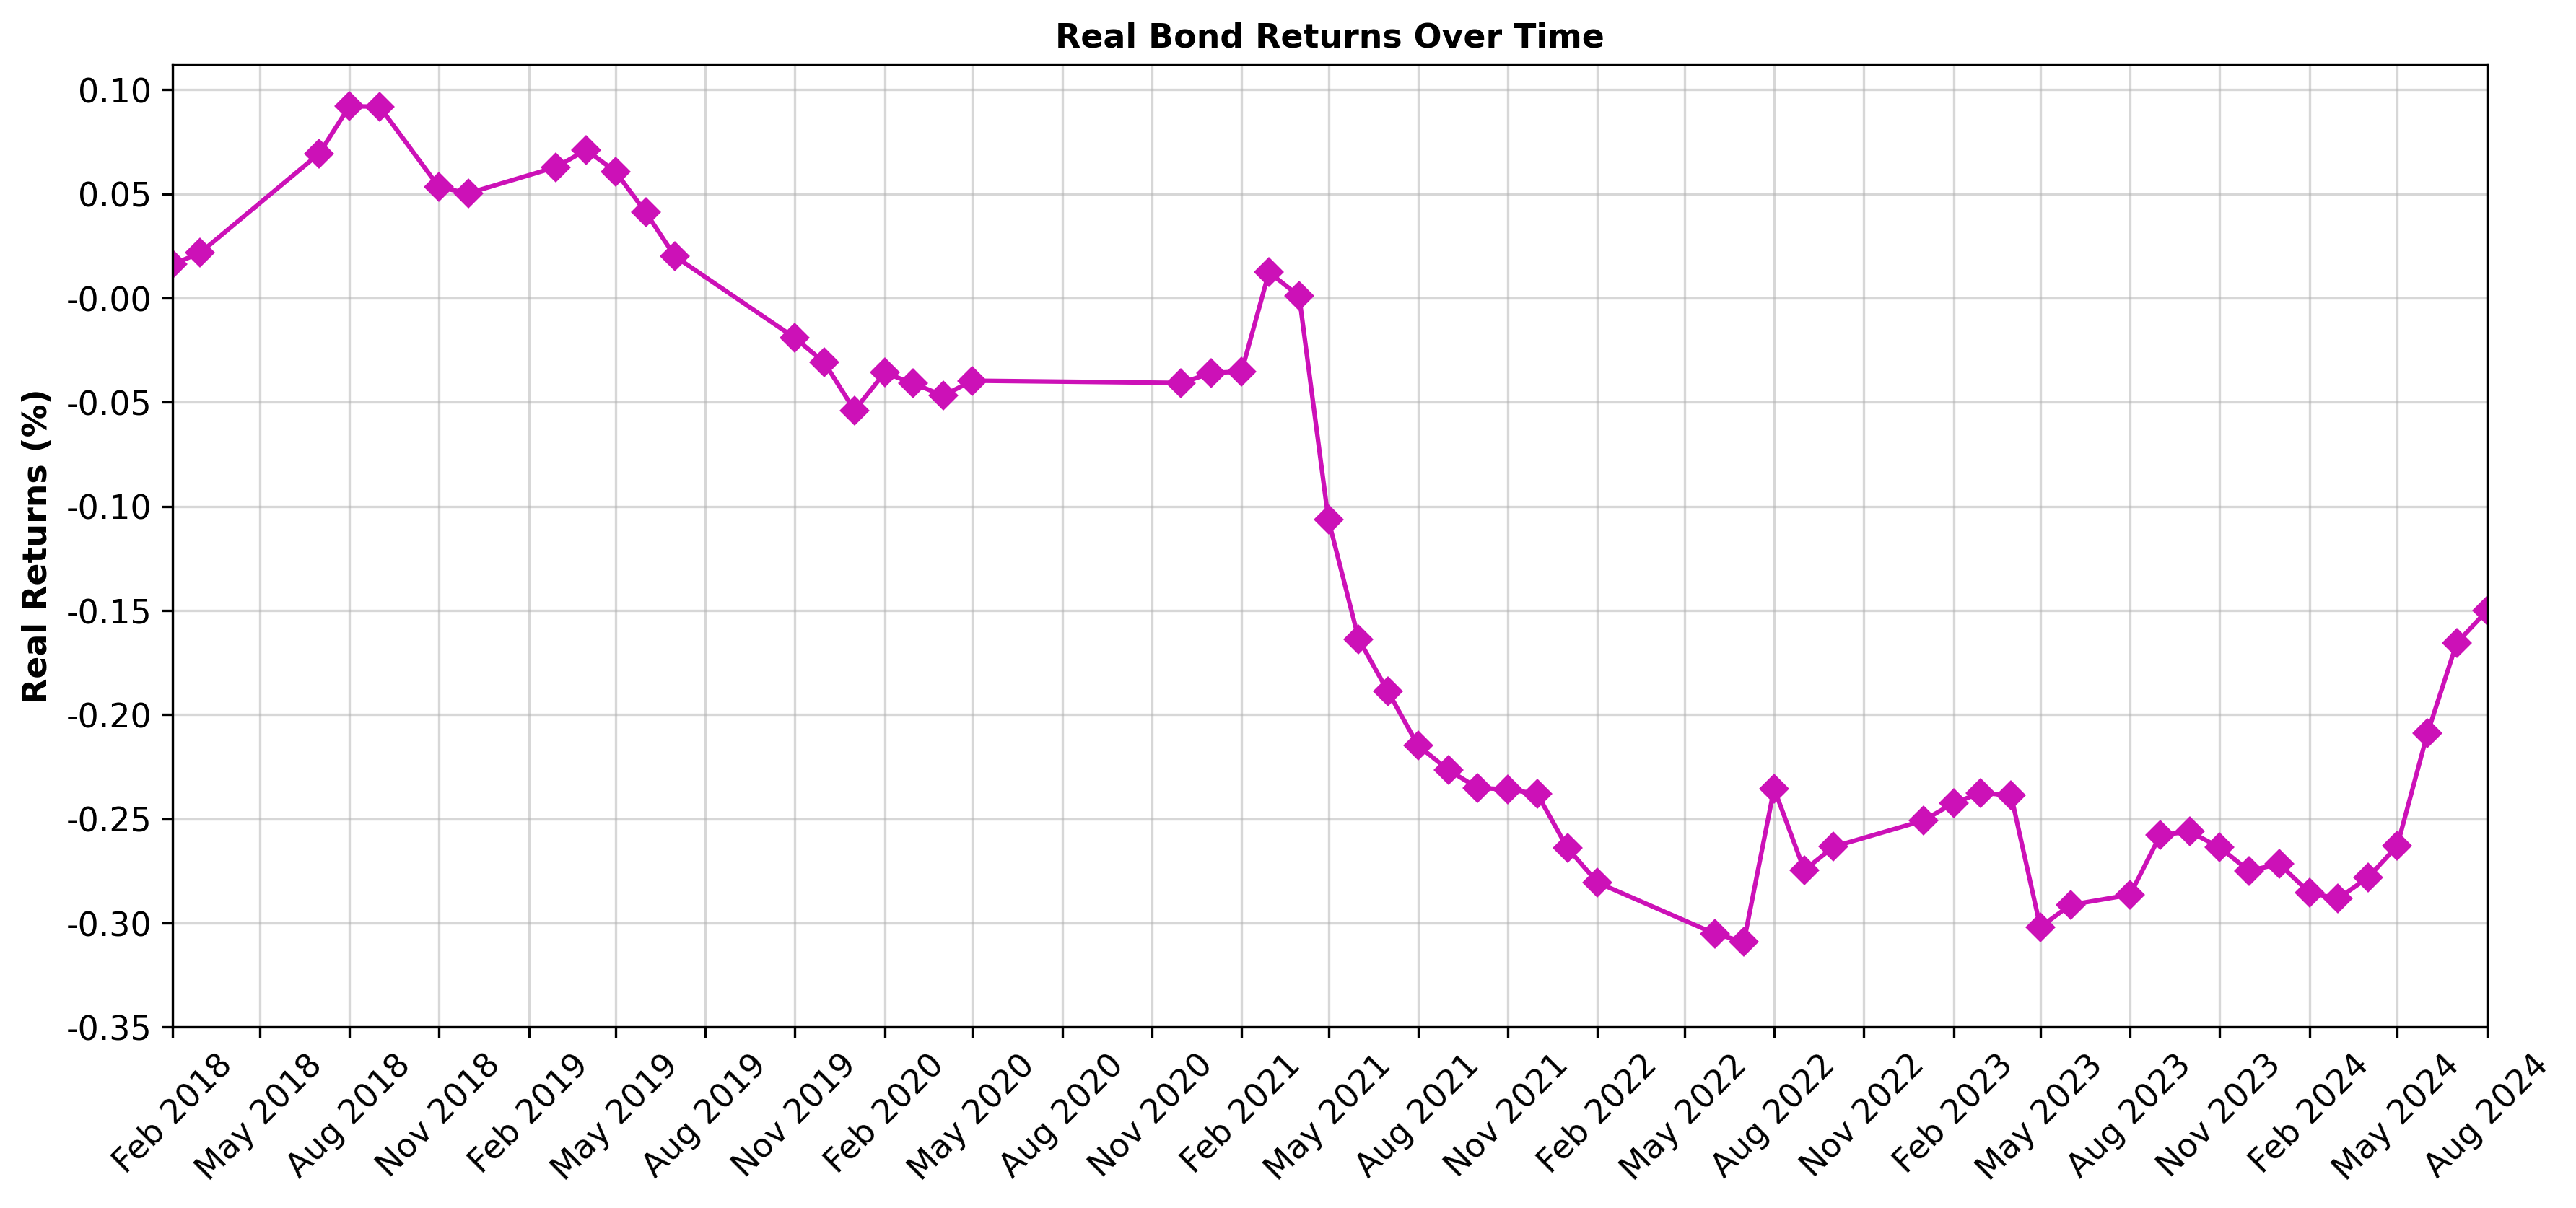
\includegraphics[width=0.7\textwidth]{real_bond_returns.png}
\begin{itemize}
\item Prolonged periods of negative real returns, especially as inflation rises.
\item Recent improvements in real returns may reflect monetary tightening, overall trend suggests that Turkish government bonds struggle to keep up with inflation.
\item Turkish bonds are not a good hedge against inflation due to their sensitivity to high inflation and credit risk.
\end{itemize}
\end{frame}

\begin{frame}{Results: Gold}
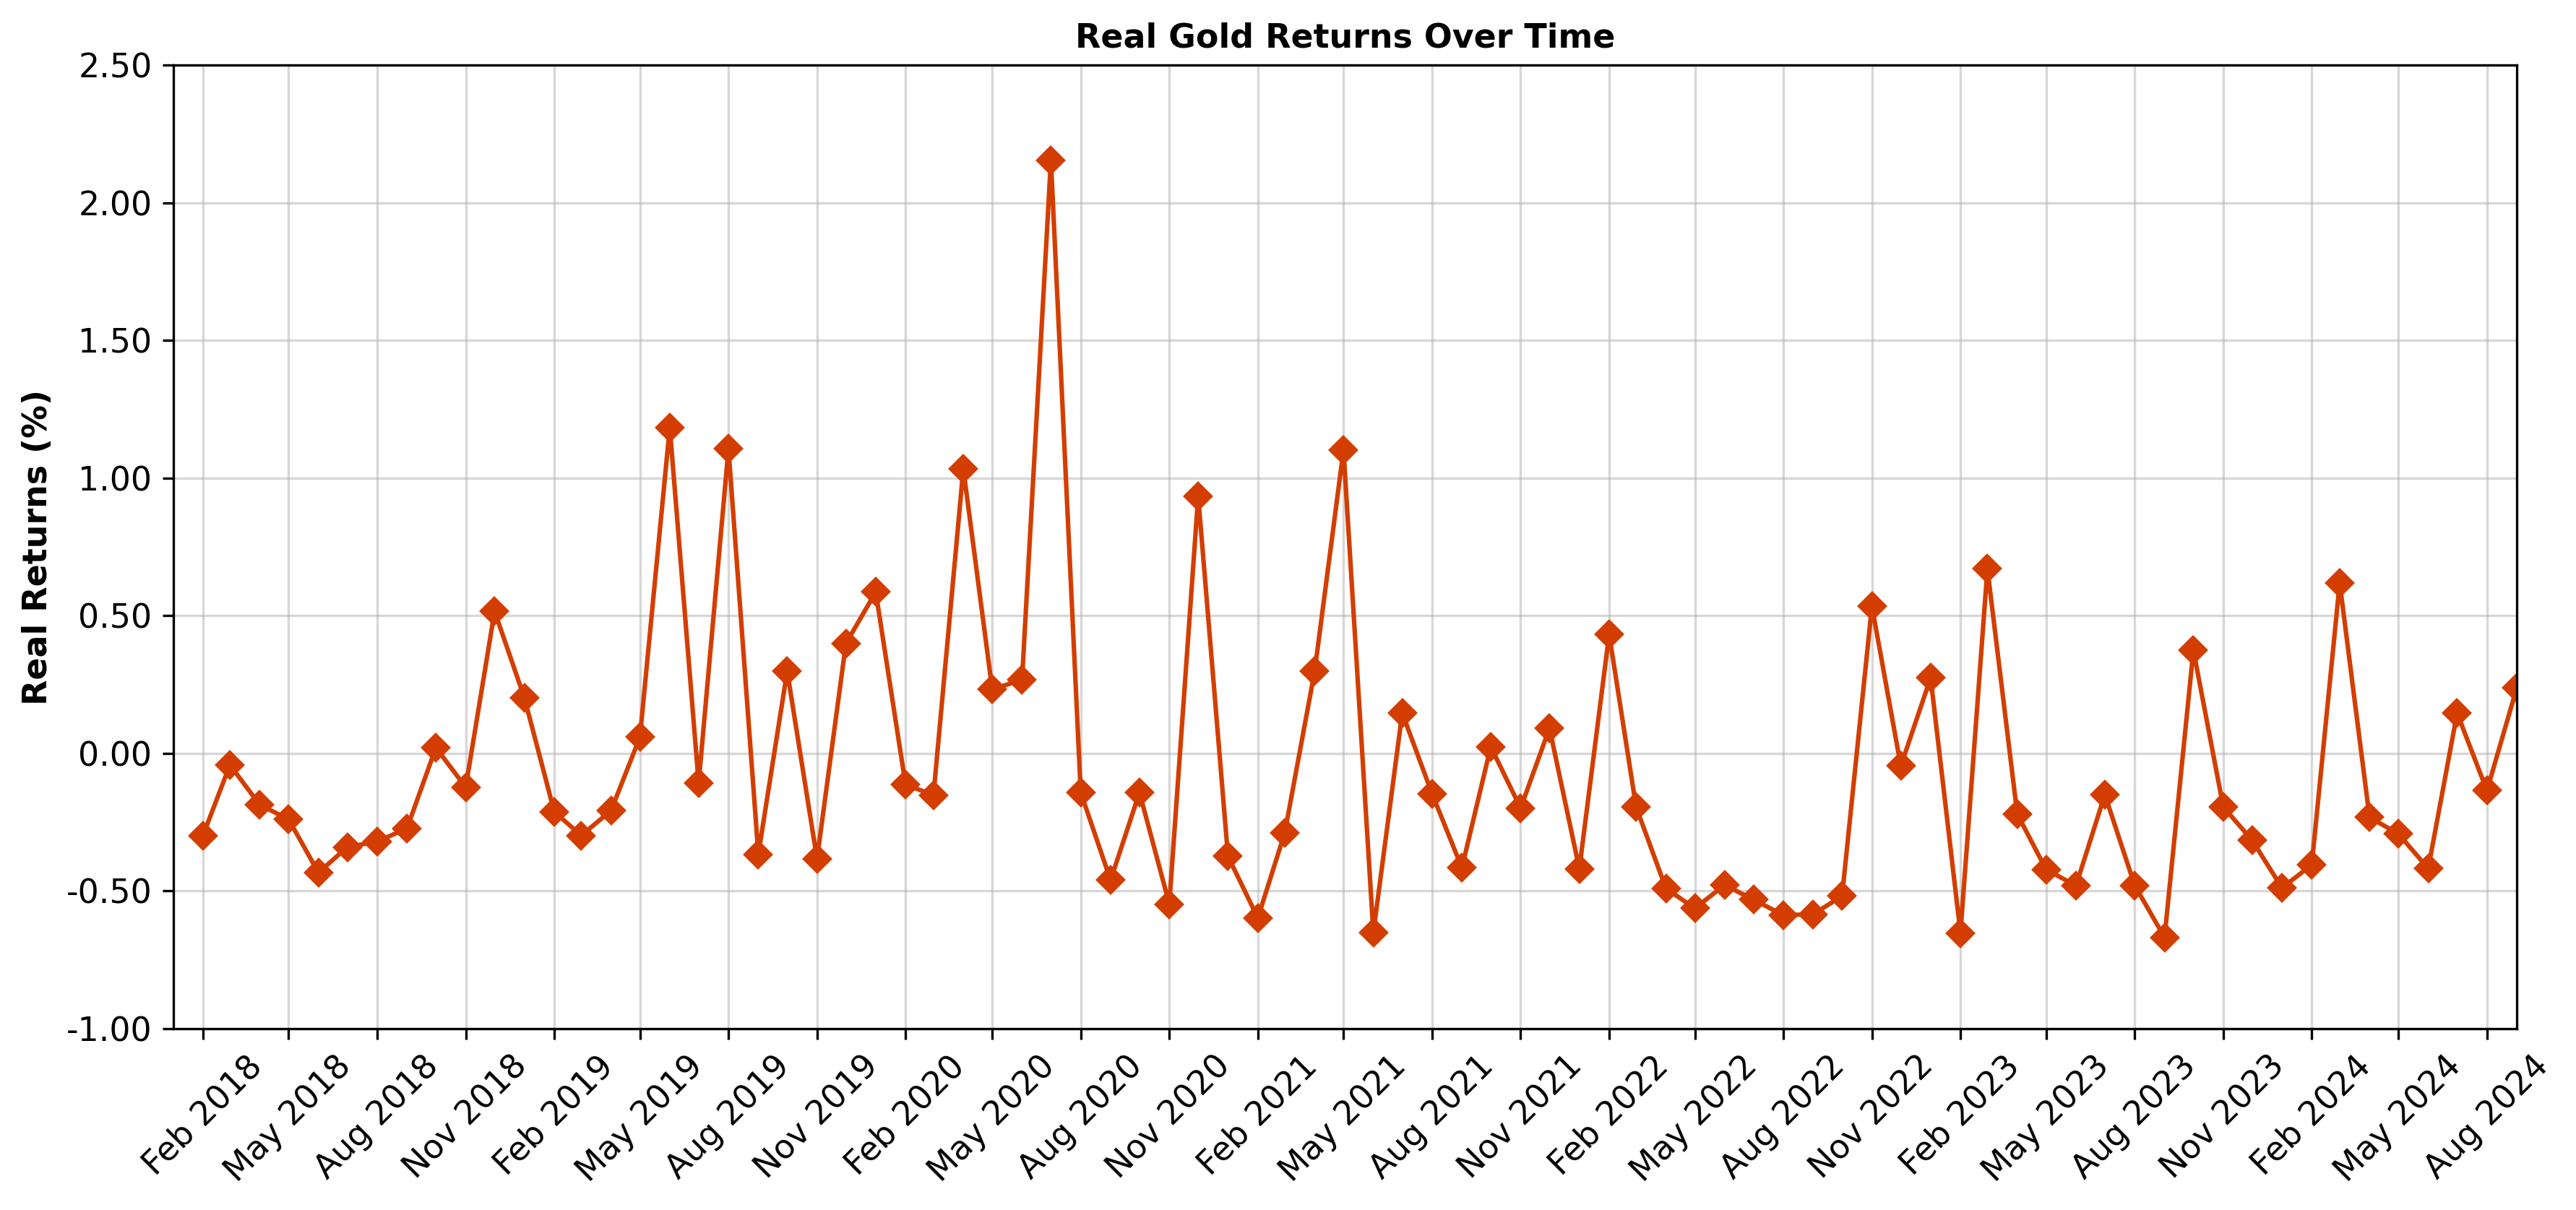
\includegraphics[width=0.7\textwidth]{real_gold_returns.png}
\begin{itemize}
\item Despite some negative returns, gold maintains a conistent performance compared to other assets.
\item This makes gold is a modest hedge against Turkish inflation, as it tends to hold its value during inflationary spikes. 
\end{itemize}
\end{frame}

\begin{frame}{Results: Bitcoin}
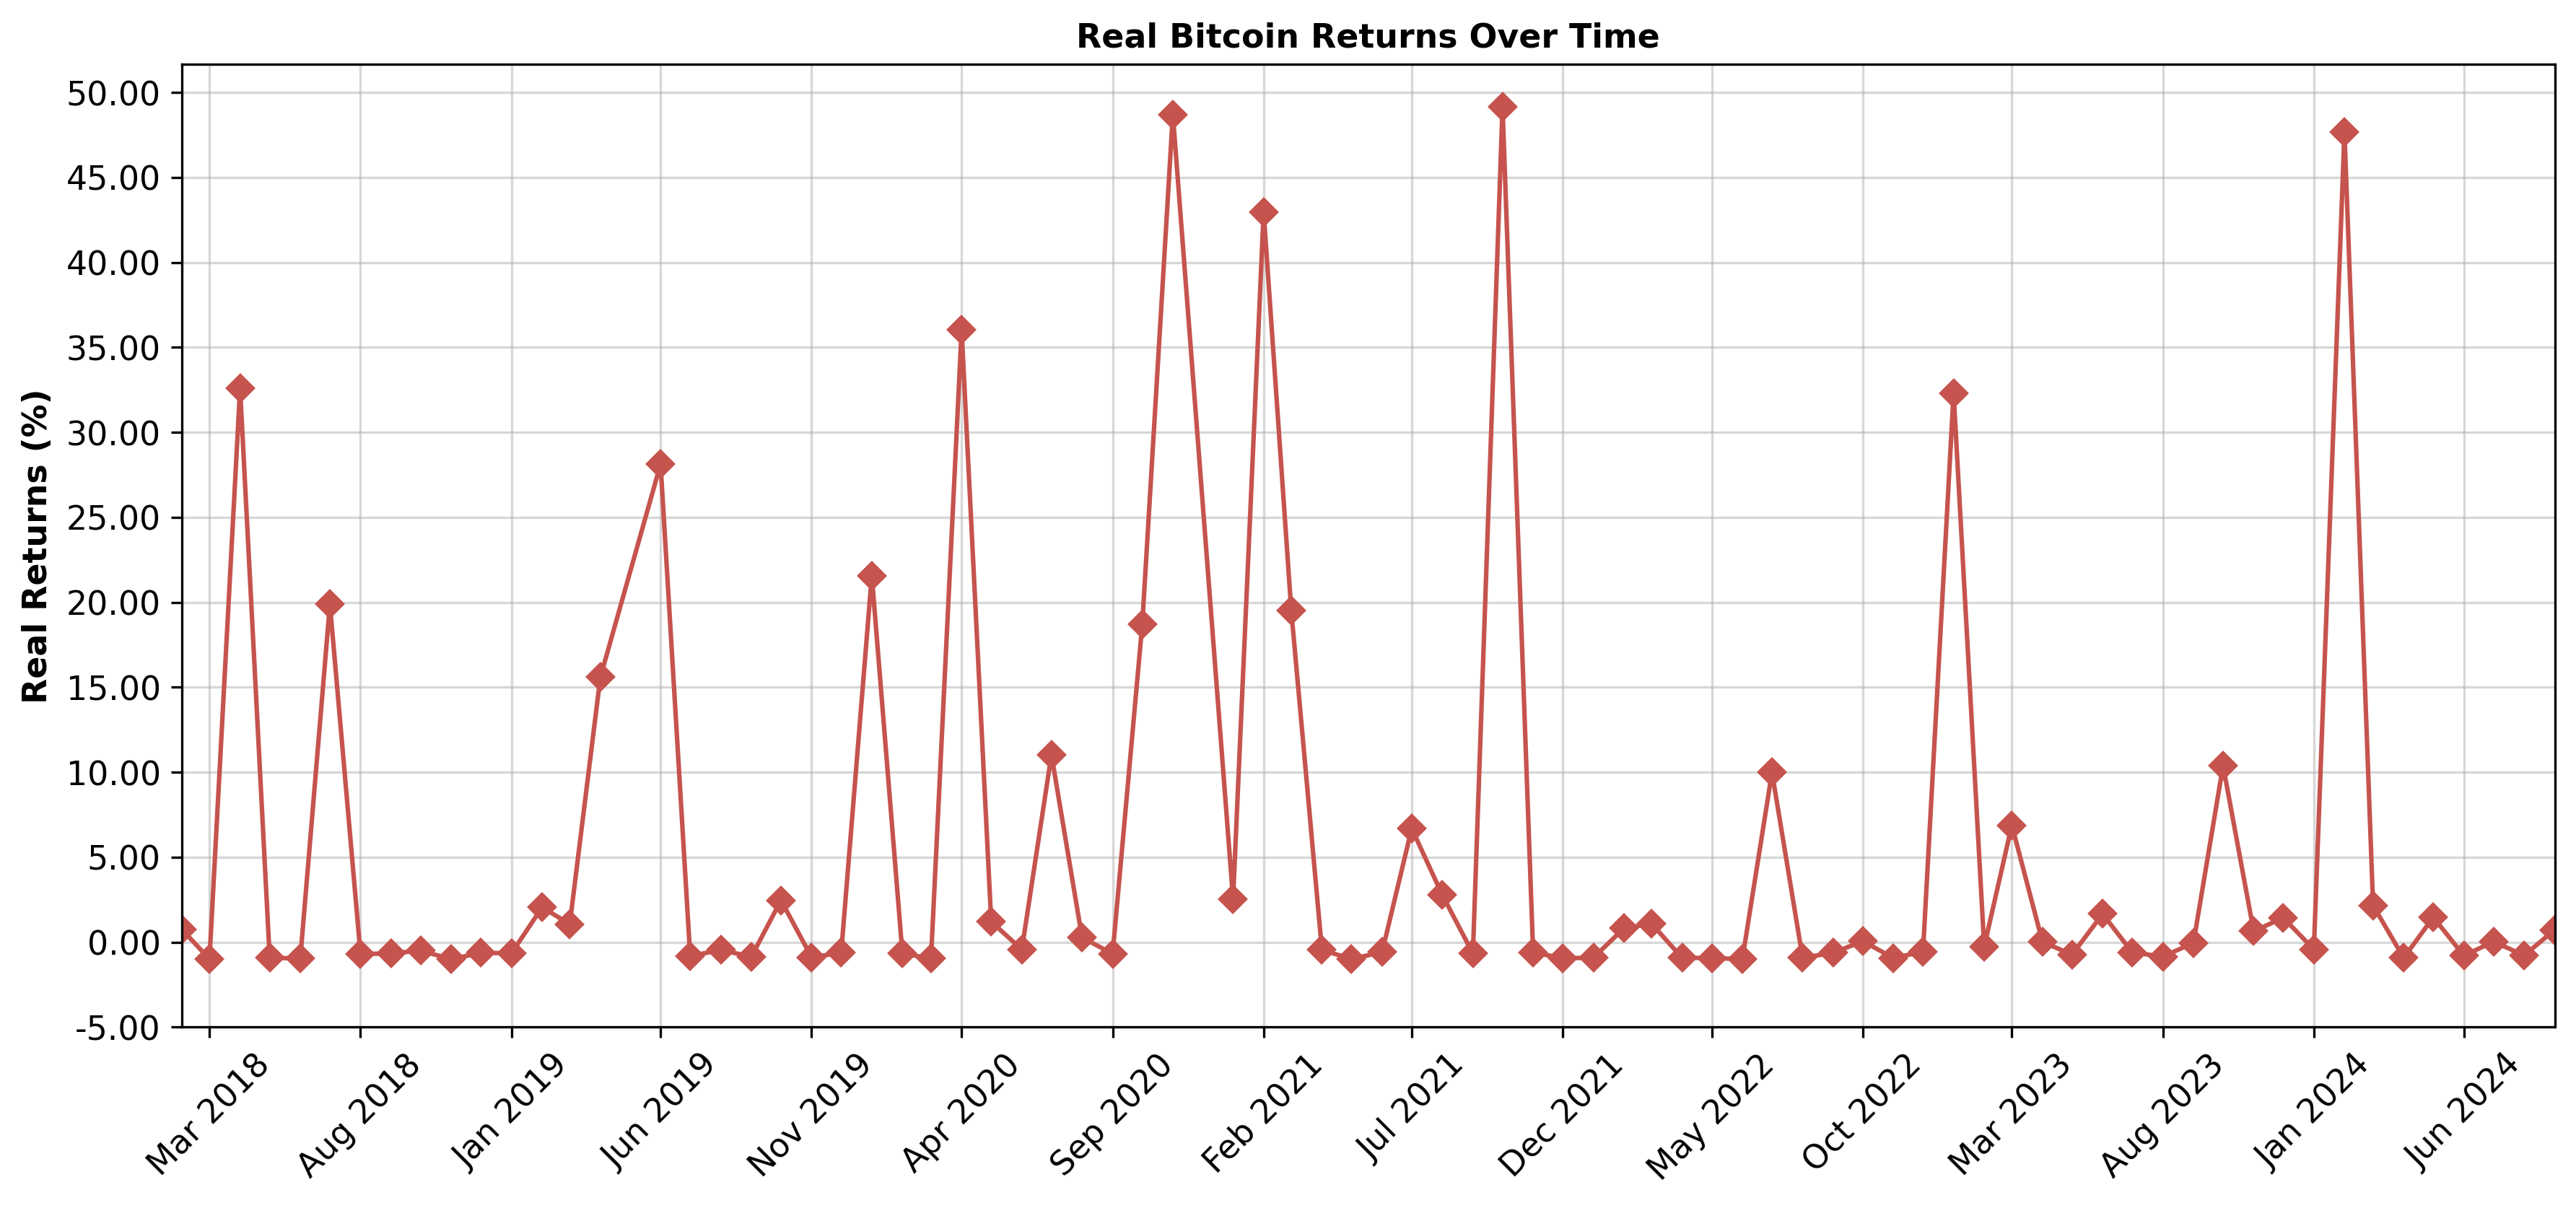
\includegraphics[width=0.7\textwidth]{real_bitcoin_returns.png}
\begin{itemize}
\item Bitcoin's real returns are highly volatile.
\item It occasionally generates high positive real returns but also shows frequent periods of near-zero or negative returns.
\item It is not a consistent hedge against Turkish inflation due to its high volatility. While it offers occasional large positive returns, it also carries significant downside risk.
\item sThis makes it speculative rather than a stable store of value in the context of inflation hedging.
\end{itemize}
\end{frame}

\begin{frame}{Results: Turkish Real Estate}
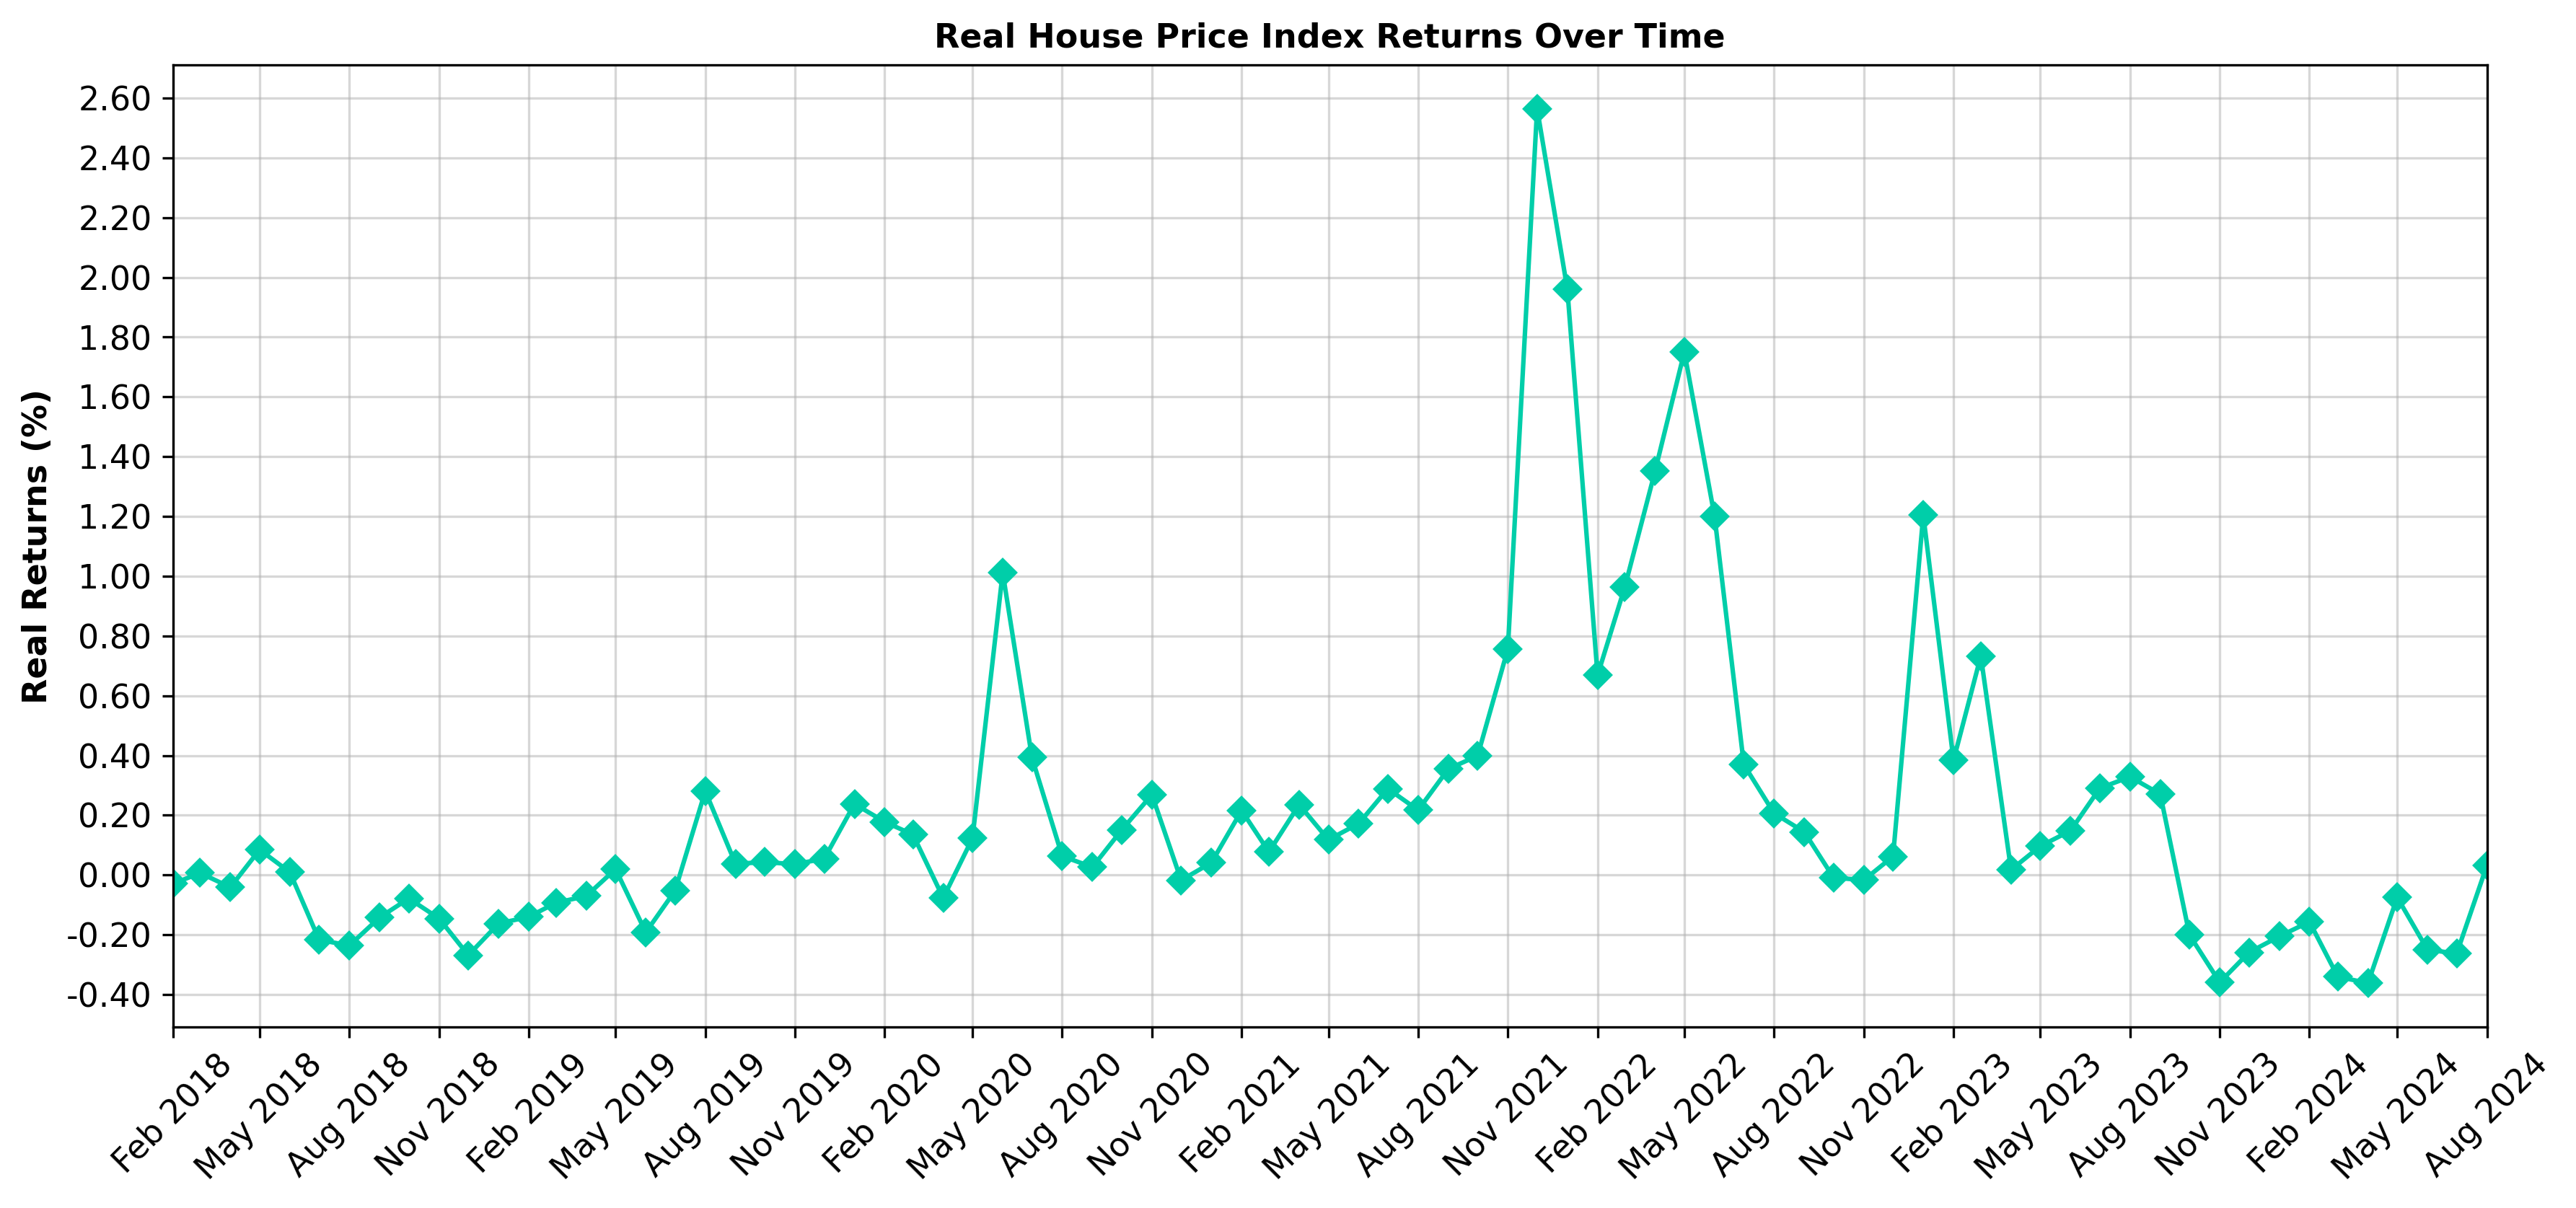
\includegraphics[width=0.7\textwidth]{real_hpi_returns.png}
\begin{itemize}
\item Real returns on Turkish real estate show occasional spikes, with also a few periods of slightly negative returns.
\item The peak in real returns occurred in late 2021, likely driven by a spike in inflation, with real estate acting as a safe haven.
\item Real estate appears to be a viable hedge against inflation during periods of high inflation in Türkiye. The sharp increase in real returns suggests strong investor demand for real assets to preserve wealth amid economic uncertainty.
\end{itemize}
\end{frame}

% Results: Markowitz Optimization
\begin{frame}{Results: Markowitz Optimization}
\begin{itemize}
    \item Using the aforementioned formula, the optimal portfolio allocation is:
    \begin{itemize}
        \item \textbf{Turkish Stocks:} 12.71\%
        \item \textbf{Turkish Government Bond:} 0.00\%
        \item \textbf{Gold:} 0.00\%
        \item \textbf{Bitcoin:} 0.92\%
        \item \textbf{Turkish Real Estate:} 86.37\%
    \end{itemize}
    \item Resulting in:
    \begin{itemize}
        \item \textbf{Expected Portfolio Return:} 35.12\%
        \item \textbf{Expected Portfolio Volatility:} 60.56\%
    \end{itemize}
\end{itemize}
\end{frame}

% Results: Markowitz Optimization
\begin{frame}{Results: Markowitz Optimization Interpretation I}
\begin{itemize}
\item Dominance of Turkish Real Estate (HPI) as the primary asset in hedging against inflation, given its historically high real returns and relatively lower risk compared to other assets.
\item Minimal allocations to Turkish Stocks (12.71\%) and Bitcoin (0.92\%) suggest that while these assets contribute to potential returns, their volatility limits their inclusion, but acts as diversification to reduce some risk.
\item Absence of Gold and Turkish Government Bonds indicates that these assets did not provide sufficient returns or diversification benefits over the period analyzed.
\end{itemize}
\end{frame}

% Results: Markowitz Optimization
\begin{frame}{Results: Markowitz Optimization Interpretation II}
\begin{itemize}
\item Expected portfolio return of 35.12\% reflects an aggressive approach that prioritizes high growth potential despite the associated risk, as indicated by the portfolio’s high volatility (60.56\%).
\item In inflationary environments, preserving purchasing power often requires accepting higher volatility.
\item Markowitz optimization is purely mathematical and does not take into account behavioral factors or practical constraints such as liquidity needs and aversion to extreme volatility. 
\end{itemize}
\end{frame}

% Conclusion
\section{Conclusion}
\begin{frame}{Conclusion}
\begin{itemize}
\item This study demonstrates that Turkish real estate is the most effective hedge against inflation over the period analyzed.
\item It also dominates the Markowitz portfolio due to its high real returns and relatively lower risk compared to other assets.
\item The resulting portfolio offers high expected returns but comes with significant volatility.
\item Future research could look into areas such as: 
\begin{itemize}
  \item Expand the asset universe to include more complex financial products, such as derivatives (e.g., inflation-linked swaps or options), exchange-traded funds (ETFs), or foreign-denominated assets. These products could provide more effective and flexible hedging mechanisms against inflation.
  \item Explore dynamic portfolio strategies that adapt to changing inflationary environments.
  \item Assess the role of alternative risk measures, such as downside risk or drawdown, to create portfolios that better address practical investor concerns.
\end{itemize}
\end{itemize}
\end{frame}

% Resources
\section{References}
\begin{frame}[allowframebreaks]{References}
\bibliography{references} % Ensure references.bib is in the same directory or update the path.
\end{frame}

\end{document}


